\chapter{基于邻域感知Transformer的知识图谱补全模型}


% 本章主要对基于邻域感知的Transformer模型NATLP的总体设计和模块的具体实现进行了介绍。主要包括对现存基于图神经网络方法存在问题的分析、模型的总体框架设计、关系特定的邻居实体信息构造设计以及融合图结构信息的自注意力机制的改进。

相较于传统的知识图谱嵌入方法,基于图神经网络的知识图谱嵌入方法通过聚合局部邻域信息获得了很大的性能提升。但是图神经网络采用的聚合方式忽略了邻居节点信息之间的潜在关联,并且模型结构较为简单。针对以上问题,本文尝试利用Transformer模型来提高模型的表达能力,完成知识图谱补全任务,提出了一种基于邻域感知Transformer的知识图谱补全模型(Neighborhood Aware Transformer for Link Prediction, NATLP)。
为了证明NATLP算法以及相关的关键设计能够有效提高知识图谱补全任务的性能,本文在两个标准数据集上进行了实验验证。本文首先对NALTP的实验方案设计进行了介绍,包括实验采用的数据集、实验环境、评估策略;用来对比的基线算法以及模型在两个数据集上的超参数设置;随后对模型的实验结果进行了分析和讨论,包括整体性能分析、关键设计分析。
% Transformer网络虽然在自然语言处理(NLP)领域取得了巨大成功,但在直接应用到图表示学习(Graph Representation Learning)领域时会遇到一系列挑战和困难。图表示学习涉及到处理图数据,图数据具有非欧几里得结构,这与NLP中处理的序列数据(一维结构)有本质区别。下面列举了一些Transformer在图表示学习中面临的主要困难:

% 1. **非序列结构**:图是一种无序的数据结构,节点之间的关系是通过边来定义的,并且没有固定的顺序。相比之下,Transformer网络原本是为处理序列数据设计的,它使用位置编码来保留序列中元素的顺序信息。在图中,节点没有自然的顺序,因此Transformer网络无法直接使用位置编码来捕捉节点间的结构关系。

% 2. **邻居多样性**:在图中,每个节点可能有不同数量的邻居。这种动态的、不规则的邻接关系与Transformer网络中假设的固定大小的输入上下文不相符。因此,直接应用自注意力机制来学习图节点表示时难以处理不同节点的可变邻居数量。

% 3. **长距离依赖**:尽管Transformer网络擅长捕捉长距离依赖,但在图中,这种依赖通常是通过节点之间的路径来定义的,而不是序列中的线性位置。因此,Transformer需要被修改或扩展,以便能够理解和利用图中的路径和结构模式。

% 4. **缩放问题**:对于大型图,使用Transformer进行全图的自注意力学习是计算资源密集型的,因为复杂度是图中节点数量的平方。这使得直接在大规模图上应用Transformer变得不切实际。

% 5. **边的信息和类型**:在图中,边可能包含重要的信息,并且边的类型(如社交网络中的不同关系类型)也可能对图表示至关重要。然而,标准的Transformer模型并没有直接的方式来编码和使用边的信息。

% 为了克服这些困难,研究人员已经提出了许多不同的方法和模型的变种,如图注意力网络(Graph Attention Networks, GATs)和图Transformer网络(Graph Transformer Networks),这些模型专门设计或修改以适应图数据的特性。这些变种通常包括对自注意力机制的修改,以更好地处理图的结构性质,以及引入适合于图结构的新型位置编码或相对位置编码。此外,为了处理大型图,研究人员还在探索如何有效地对图进行采样,以及如何利用稀疏性和分层结构来降低计算复杂度。

% Transformer在知识图谱嵌入任务中具有以下优点:

% 1. 处理长距离依赖关系:知识图谱中的实体和关系之间存在着复杂的长距离依赖关系。传统的基于图的模型(如Graph Convolutional Networks)往往只考虑局部邻居信息,难以捕捉到远距离的语义依赖。而Transformer通过自注意力机制可以处理全局上的依赖关系,能够更好地捕捉实体和关系之间的长距离语义关联。

% 2. 并行计算能力:与循环神经网络不同,Transformer网络可以进行并行计算,加快了训练和推理的速度。在大规模的知识图谱中,由于实体和关系的数量庞大,传统的基于图的模型可能面临计算效率低下的问题,而Transformer网络能够更高效地处理大规模的知识图谱数据。

% 3. 对复杂属性建模:知识图谱中的实体通常具有丰富的属性信息,如文本描述、分类标签等。传统的基于图的模型往往无法有效地捕捉和利用这些属性信息,而Transformer网络可以将这些属性信息作为输入,并通过多头注意力机制对不同属性进行建模,从而更好地捕捉实体的语义特征。

% 4. 高度可扩展性:Transformer网络可以通过增加层数和调整参数来提高模型的表示能力。在知识图谱嵌入任务中,复杂的语义关系和多层次的结构需要一个具有较强建模能力的模型来学习。Transformer网络的多层结构可以提供更强的表示能力,可以通过增加层数来适应不同任务的需求。

% 综上所述,Transformer在知识图谱嵌入任务中具有处理长距离依赖关系、并行计算能力、对复杂属性建模和高度可扩展性等优点,为知识图谱的表示学习提供了一种强大而灵活的模型选择。

%注意力中添加度数:1-1/度数乘积

\section{现有问题描述和分析}

图卷积神经网络GCN于2017年被提出,对原先图神经网络中基于谱空间的的图卷积算子进行了优化,降低了模型的复杂度,由此引发了图神经网络的研究热潮。图神经网络迅速成为了图结构数据处理的重要方式,在社交网络\upcite{social}、推荐系统、知识图谱等多个领域都有着重要应用。近几年,图神经网络的应用是知识图谱嵌入领域非常重要的进展。图卷积神经网络能够直接处理图结构数据并捕捉知识图谱中的拓扑结构,通过聚合邻居节点的信息,图神经网络可以有效地学习知识图谱中节点(实体)和边(关系的嵌入表示)。相较于之前的方法,基于图神经网络的知识图谱嵌入方法获得了很大的性能提升。

然而,受限于本身的网络结构,在进行知识图谱嵌入时,基于图神经网络的方法依然存在不足,导致其性能受限。首先,图卷积神经网络采用聚合邻居节点的方法来更新中心实体的表示,在这个过程中,模型只考虑了邻居节点和中心实体之间的连通性,却忽略了不同邻居节点之间的可能也存在直接连接,各个邻居节点传递的信息之间是互不感知、互相独立的,这样的聚合方式没有将邻居节点信息之间的相互依赖纳入考虑;其次,图神经网络采用的消息传递模式整体模型结构比较简单,使模型的表达能力受到了限制,在挖掘图谱中实体和实体、实体与关系之间的复杂交互上存在困难。

而在以上两个方面,Transformer网络存在巨大的优势。首先,通过构造查询向量、键向量和值向量来进行注意力的计算以及采用多头注意力机制,相比于图神经网络,Transformer能够更加高效地挖掘输入之间各个维度的复杂交互;同时,通过调整模型的层数、头的数量或是隐层的维度大小,Transformer可以很容易地适应处理不同规模和复杂度的知识图谱的需求。

其次,Transformer网络的自注意力机制能够有效地捕捉序列中任意两个元素之间的全局依赖关系。在知识图谱嵌入的场景之中,这意味着模型在挖掘局部邻域的结构信息时,除了邻居节点和中心节点之间的依赖之外,还能够同时学习到邻居节点之间的依赖,捕获邻居节点传递的信息之间的相互影响。此外,Transformer架构还支持模型的预训练和迁移学习,可以首先在一个大规模的综合性知识图谱上进行预训练,然后迁移到特定领域的知识图谱上,通过这样的方式,可以减少模型对标注数据的依赖,提高模型在特定任务上的表现。

虽然Transformer网络在自然语言处理(NLP)领域已经取得了巨大成功,但将Transformer网络直接应用到知识图谱嵌入领域时依旧会遇到一系列挑战和困难。图具有非欧几里得结构,是一种无序的数据结构,这与NLP中处理的序列数据(一维结构)有本质区别。Transformer网络原本是为处理序列数据设计的,它使用位置编码来保留序列中元素的顺序信息。但是,在知识图谱中,节点之间的关系是通过边来定义的,并且没有固定的顺序,因此Transformer网络无法直接使用位置编码来捕捉节点间的相对位置关系,需要对输入进行一些额外的预处理或者对Transformer进行一些改造,在这个过程中容易出现结构信息的失真。部分使用了Transformer网络的方法例如MAGNN\upcite{MAGNN}选择通过随机游走的方式来将图数据转化为序列数据来处理,这样的方式导致模型丢失了对图结构的感知。

此外,在知识图谱中,边,即关系,反映着实体和实体之间不同的交互方式,蕴含着丰富的语义信息。两个实体之间连接的关系不同,传递的信息可能是千差万别的,因此如何采用合适的方式来对利用关系信息,体现关系对于消息传递的影响十分重要。但标准的Transformer模型并没有直接的方式来编码和使用边的信息。部分利用Transformer来进行知识图谱表示学习的模型例如Relphormer\upcite{Relphormer}将知识图谱中的实体和关系视为地位相同的节点,采用同样的方式进行处理,这样的方式虽然解决了边的表示问题,但没有考虑到知识图谱中实体和关系的差异性,没有考虑到关系对于实体消息传递的独特作用。

为了解决上述问题,本章提出了一种基于邻域感知Transformer的知识图谱补全模型(Neighborhood Aware Transformer for Link Prediction, NATLP)。首先,在模型输入信息构造阶段,为了充分建模不同关系对于实体传递消息的影响,模型基于关系生成特定的网络参数,实现关系特定的邻居信息构造。其次,为了让Transformer能够更好地处理图结构数据,模型对Transformer的自注意力机制进行了改造,提出了一种融合图结构的自注意力机制,使得Transformer能够学习到输入消息之间的互相依赖。

\section{NATLP模型设计}

\subsection{符号定义}

为了方便说明论文提出的NATLP模型的实现细节,本节首先对模型中的关键概念和相关的数学符号进行了定义,具体内容参见表\ref{definition}。

\setlength{\tabcolsep}{20pt}

\renewcommand\arraystretch{1.2}
\begin{longtable}[htbp]{cc}
  % 首页表头
  \caption{NATLP模型中的符号定义}
  \label{definition}\\
  \toprule
  符号  & 说明\\
  \midrule
  \endfirsthead
  % 续页表头
  \caption{NATLP模型中的符号定义}\\
  \toprule
  符号  & 说明 \\
  \midrule
  \endhead
  % 首页表尾
  \hline
  % \multicolumn{2}{r}{\small 续下页}
  \endfoot
  % 续页表尾
  \bottomrule
  \endlastfoot
  
  $\mathcal{G}$   &   知识图谱      \\
  $\mathcal{E}, \mathcal{R}, \mathcal{T}$   &   实体集合、关系集合、边集合      \\
  $\mathcal{G}^\prime$  &  拓展后的知识图谱      \\
  $\mathcal{R}^{\prime}$   &   拓展后的关系集合      \\
  $\mathcal{T}^{-1}$   &   逆关系边集合      \\
  $\mathcal{T}^{\prime}$   &   拓展后的边集合      \\
  $(s,r,?)$  &   待遇测的三元组      \\
  $s$   &   头实体即中心实体      \\
  $o$   &   尾实体即目标实体      \\
  $e$   &   实体      \\
  $r$   &   关系      \\
  $r^{-1}$   &   关系$r$的逆关系      \\
  $\boldsymbol{s},\boldsymbol{o}$ & 头实体嵌入和尾实体嵌入\\
  $\boldsymbol{e},\boldsymbol{r}$ & 实体嵌入和关系嵌入\\
  $d$ &嵌入维度\\
  $\phi_{chk}$ & 棋盘式特征重组\\
  $\circledast$ & 循环卷积操作\\
  $f(\cdot )$ & ReLU激活函数\\
  $vec(\cdot)$ & 二维张量转化为一维向量\\
  $k_{size}$ &卷积核的边长\\
  $n_{conv}$ &卷积核的数量\\
  $\omega_r$ & 特定于关系$r$的卷积层参数\\
  $\mathbf{W}_r$ &特定于关系$r$的全连接层参数\\
  $\mathbf{W}_{conv}$ & 卷积层参数生成网络\\
  $\mathbf{W}_{fc}$ & 全连接层参数生成网络\\
  $\boldsymbol{r}_{global}$ & 全局关系嵌入\\
  $\mbox{Re3D}(\cdot)$ & 一维向量转化为三维张量\\
  $\mbox{Re2D}(\cdot)$ & 一维向量转化为二维张量\\
  $\boldsymbol{m}_{e,r}$ & 邻居实体$e$通过关系$r$传递的信息\\
  $\boldsymbol{e}_{cls}$ & 特殊嵌入Class Token\\
  $\mathbf{TE}$ & 类型嵌入\\
  $a_{ij}$ & 第i个输入和第j个输入之间的注意力得分\\
  $dis(e_i,e_j)$ & 实体$e_i$与实体$e_j$之间最短路径的距离\\
  $deg(e)$ & 实体$e$的节点度数\\
  $\boldsymbol{o}_t$ & 模型预测的候选实体的嵌入\\
  $\ast $ & 普通卷积操作\\
  $\sigma $ & sigmoid激活函数\\
  $p$ & 三元组正确概率\\
  $L$ & 模型损失\\
  $t_i$ & 第i个三元组的标签\\

\end{longtable}

知识图谱是表示为$(s,r,o)$的“头实体-关系-尾实体”事实三元组的集合,所有的这些事实三元组连接起来构成了一个异构图,即为知识图谱,表示为$\mathcal{G} = (\mathcal{E}, \mathcal{R}, \mathcal{T})$,其中$\mathcal{E}$集合,$\mathcal{R}$为关系集合,$\mathcal{R}$为实体和关系构成的边集合。由于知识图谱中的关系具有方向性,为了确保信息能够在两个相连的实体之间进行双向的流通,本文在知识图谱中为每个事实三元组$(s,r,o)$创建了对应的逆三元组$(o,r^{-1},s)$,其中$r^{-1}$是关系$r$对应的逆关系。因此,关系集合、边集合以及知识图谱被拓展为:
\begin{gather}
    \mathcal{R}^{\prime}=\mathcal{R}\cup\{ r^{-1} | r\in \mathcal{R}\}\\
    \mathcal{T}^{-1}= \{ (o,r^{-1},s)| (s,r,o)\in \mathcal{T}\}\\
    \mathcal{T}^{\prime} = \mathcal{T}\cup\mathcal{T}^{-1}\\
    \mathcal{G}^\prime = (\mathcal{E}, \mathcal{R}^\prime, \mathcal{T}^\prime)
\end{gather}

知识图谱补全任务,即链路预测任务,是在给定待预测三元组中的头实体$s$以及关系$r$的情况下预测缺失的尾实体$o$,表示为$(s, r, ?)$,或者是在给定尾实体$o$以及逆关系$r^{-1}$的情况下预测缺失的头实体$s$,表示为$(?, r^{-1} , o) $。为了方便说明,论文随后统一采用$(s, r, ?)$的形式进行表述。


\subsection{模型总体结构}

本节主要对提出的用于链路预测的基于邻域感知Transformer的知识图谱补全模型NATLP的总体结构进行介绍。NATLP整体为编码器-解码器架构,编码器部分主要由关系特定的邻居信息构造模块和邻域感知Transformer模块组成,解码器部分则采用了基于卷积神经网络的知识图谱嵌入方法进行了实现。模型整体架构如图\ref{architecture}所示。

\begin{figure}[htb]
  \centerline{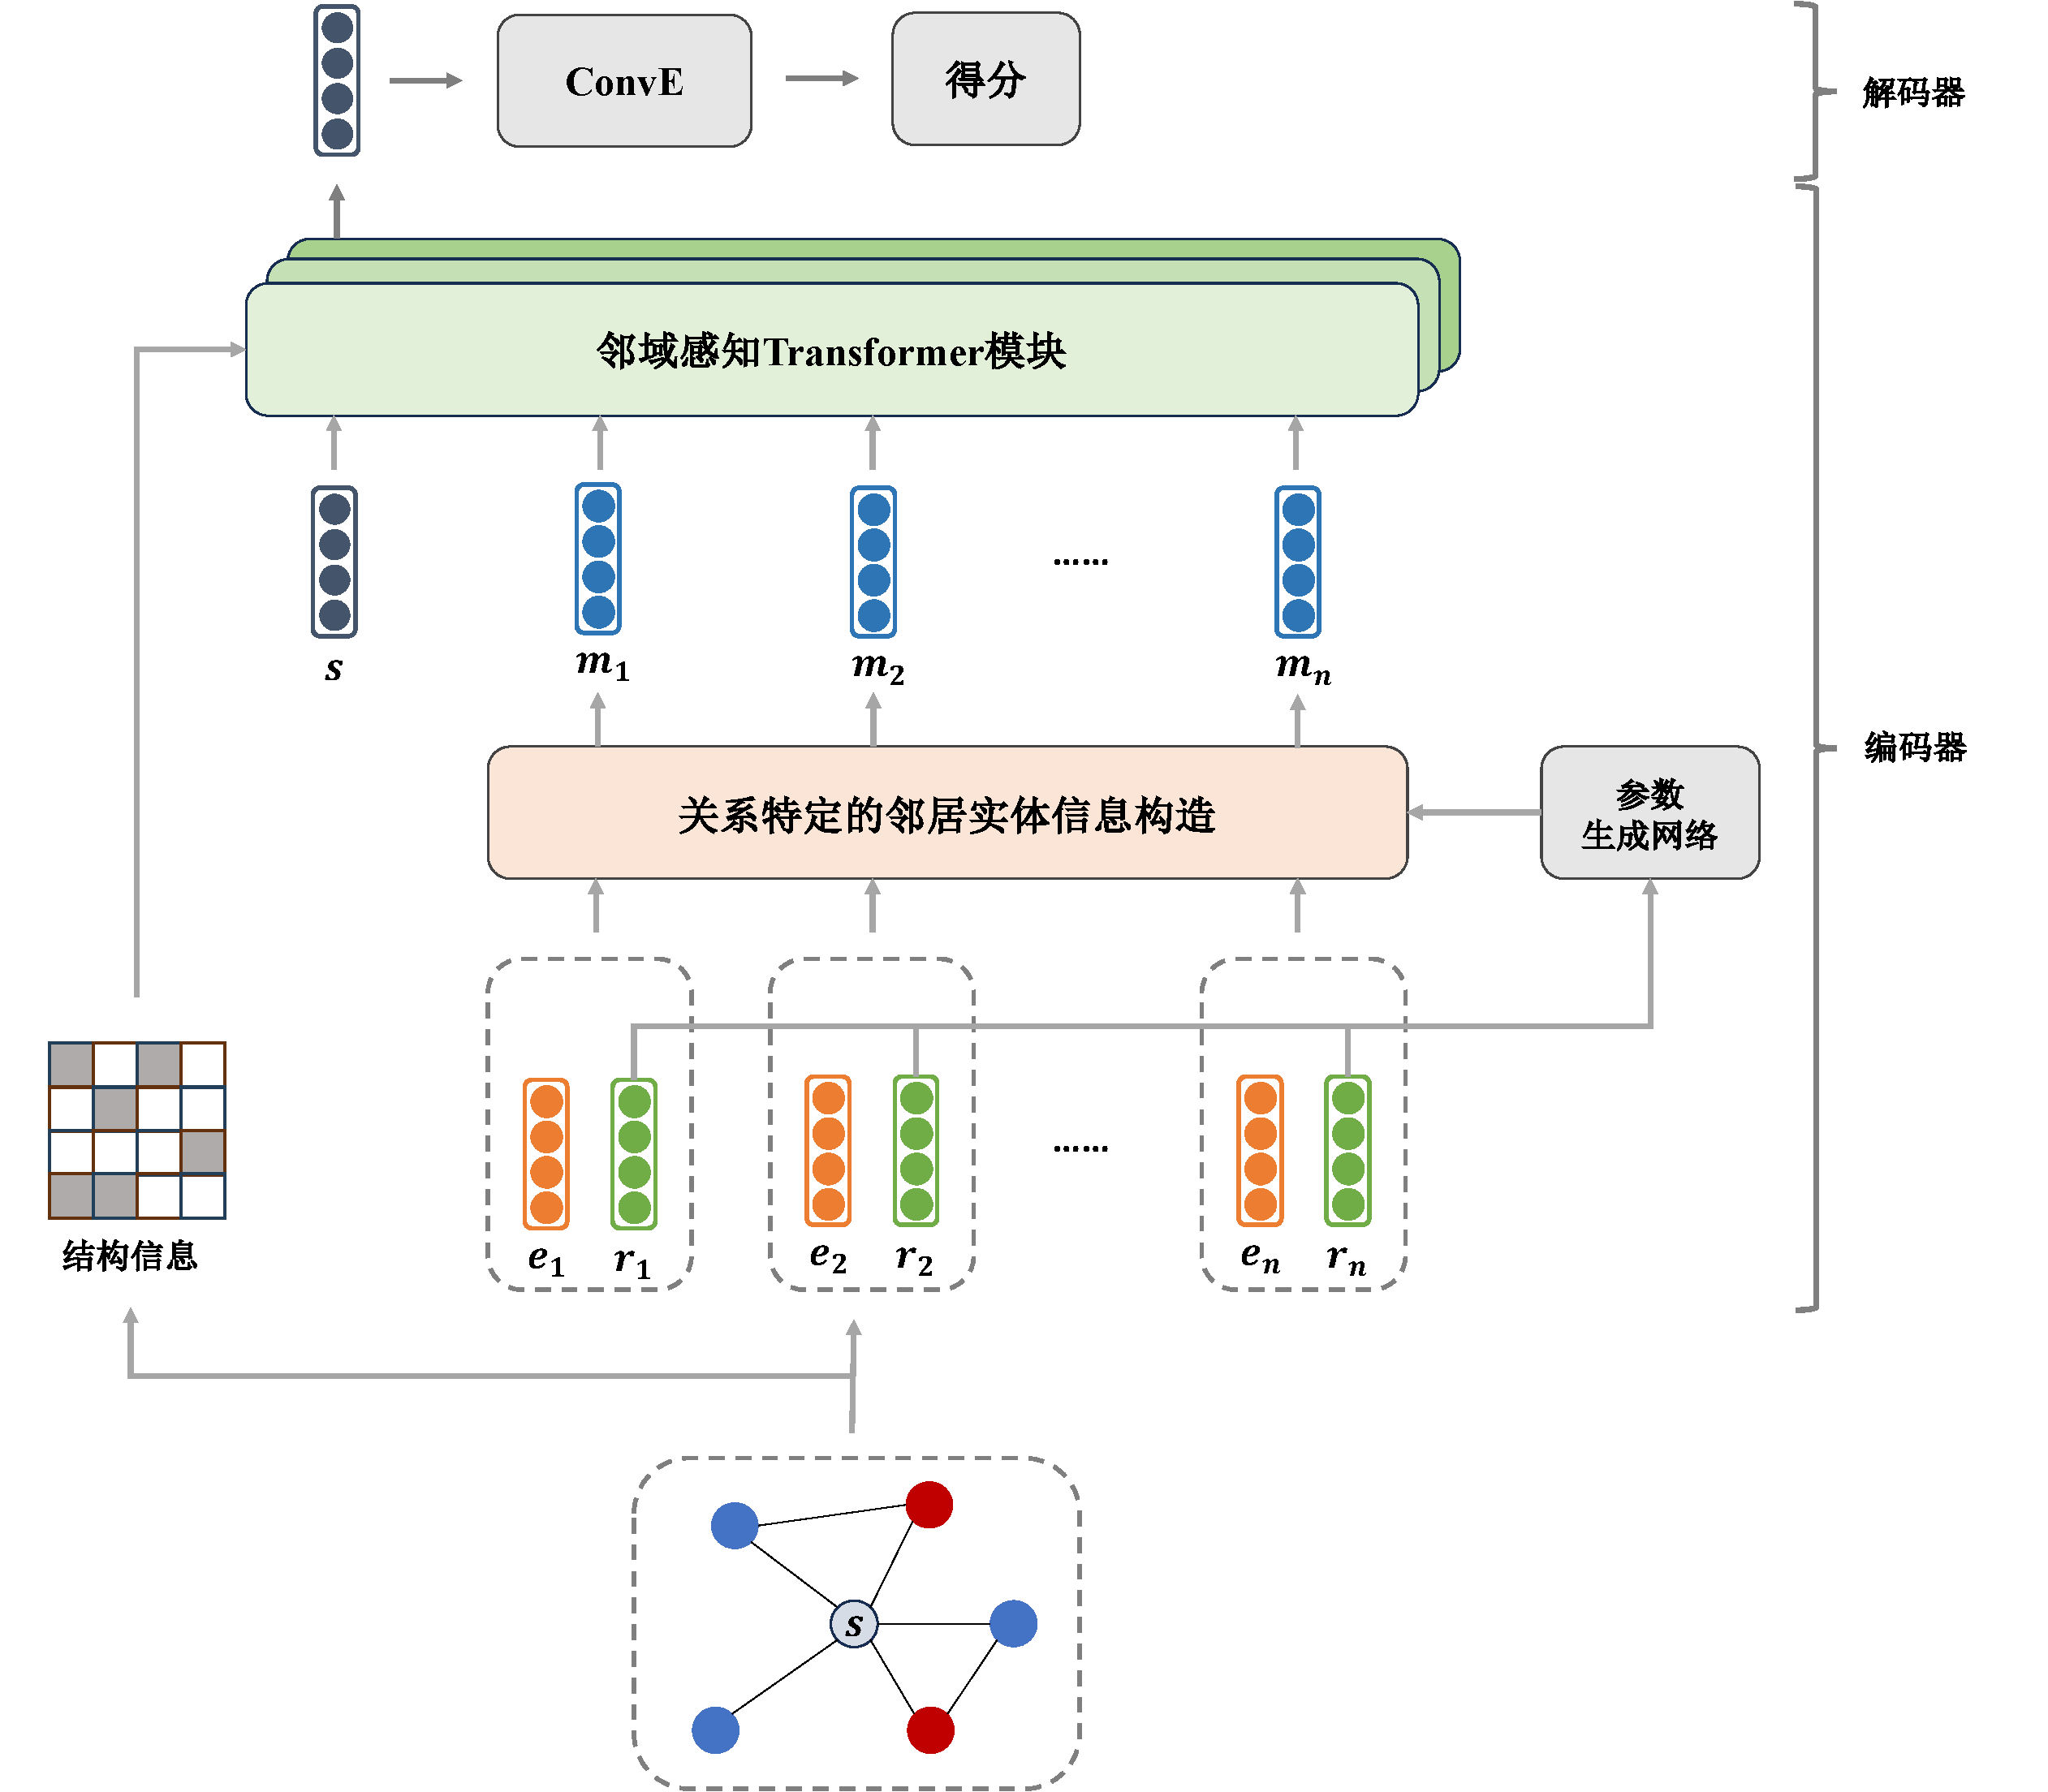
\includegraphics[width=0.9\textwidth]{pic/architecture.pdf}}
  \caption{NATLP模型整体架构}
  \label{architecture}
\end{figure}

编码器的主要作用是将模型输入的实体和关系转化为对应的嵌入,并学习其中蕴含的语义信息和结构信息并编码成向量形式,是模型的核心部分。在NATLP中,模型的输入主要包括待预测的三元组及其局部邻域,编码器首先会根据中心实体和邻居之间相连的关系种类,为每一个邻居实体构造关系特定的邻居消息;随后的邻域感知Transformer模块综合学习构造的邻居信息、中心实体本身的信息以及局部邻域的结构信息,并完成编码。

解码器的主要任务则是根据编码器得到的知识表示,对下游任务的各项性能指标进行评测。根据下游任务的不同,模型可以采用不同的解码器进行解码。NATLP采用了基于卷积神经网络的知识图谱嵌入方法ConvE作为解码器,来对事实三元组的正确概率进行评估,完成知识图谱补全。

\subsection{关系特定的邻居实体信息构造}

链路预测任务的目标是利用知识图谱中已有的事实去预测未知事实在知识图谱中的存在概率。为了能够充分利用邻域信息来帮助预测三元组中缺失的尾实体,NATLP需要获得局部邻域中邻居实体向中心实体传递的信息。知识图谱中的关系反映着实体和实体之间不同的交互方式,但标准的Transformer模型没有办法直接对关系进行编码。为了解决这个问题,受到基于图神经网络的知识图谱嵌入方法中的消息传递模型的启发,NATLP首先基于连接的关系完成邻居实体的消息构造后,再将消息传递到Transformer模型中进行学习。

但是,目前基于图神经网络的知识图谱嵌入方法中采用的消息构造函数存在着一些不足。本文调研了部分基于图神经网络的知识图谱嵌入方法采用的消息构造函数,具体内容见表\ref{message_Function}。

可以发现,除了R-GCN\upcite{R-GCN}之外,其余的方法对于实体通过不同关系传递的信息,采用的都是同样的网络参数进行编码。但是,同一个实体和不同的关系相连,表达的语义信息可能完全不一样。例如(姚明,出生于,上海)和(姚明,职业,篮球运动员),传递的信息就有着很大不同。采用同样的参数进行编码,会导致模型难以捕获实体中的和不同关系相关的特定特征。针对关系的这个特点,R-GCN模型为每个关系都定义了单独的网络参数,但是这样的方法也存在问题:一方面,每类关系的网络参数需要单独进行学习,对于数量较少的关系可能会出现训练不充分的情况;另一方面,这样的方法会容易导致关系之间的内在相关性被忽略。TransCoRe\upcite{TransCoRe}对TransE/TransH/TransR学习到的关系嵌入进行了分析,发现关系之间的相关性通过嵌入表示上的低秩结构显示出来,即不同种类的关系之间存在某种共同的特点。

\begin{table}[htbp]
    \renewcommand\arraystretch{1.5}
    \caption{部分基于图神经网络的知识图谱嵌入方法采用的消息构造函数}
    \label{message_Function}
    \centering
    \begin{tabular}{cc}
      \toprule
      知识图谱嵌入方法 & 采用的消息构造函数\\
      \midrule
      R-GCN\upcite{R-GCN} & $\mathbf{W}_re$\\
      SACN\upcite{SACN} & $\mathbf{W}e$\\
      Graph2Seq\upcite{Graph2Seq} & $\mathbf{W}_{in}\left[e_i,r_k,e_j\right] \ \mbox{or} \ \mathbf{W}_{out}\left[e_i, r_k, e_j\right]$\\
      CompGCN\upcite{CompGCN} & $\mathbf{W}_{dir(r)}e_i\star e_k$\\
      KBGAT\upcite{KBGAT} & $\mathbf{W}\left[e_i, e_j, r_k\right] $\\
      RGHAT\upcite{RGHAT} & $\mathbf{W}_2\left[\mathbf{W}_1\left[e_i, r\right], e_j\right]$\\
      \bottomrule
    \end{tabular}
  \end{table}

为了解决上述问题,实现捕获邻居实体中关系相关的特定特征的同时,兼顾不同类别关系之间的共通特征,NATLP提出了一种关系特定的邻居实体信息构造方法,具体如图\ref{build_information}所示。

\begin{figure}[htb]
  \centerline{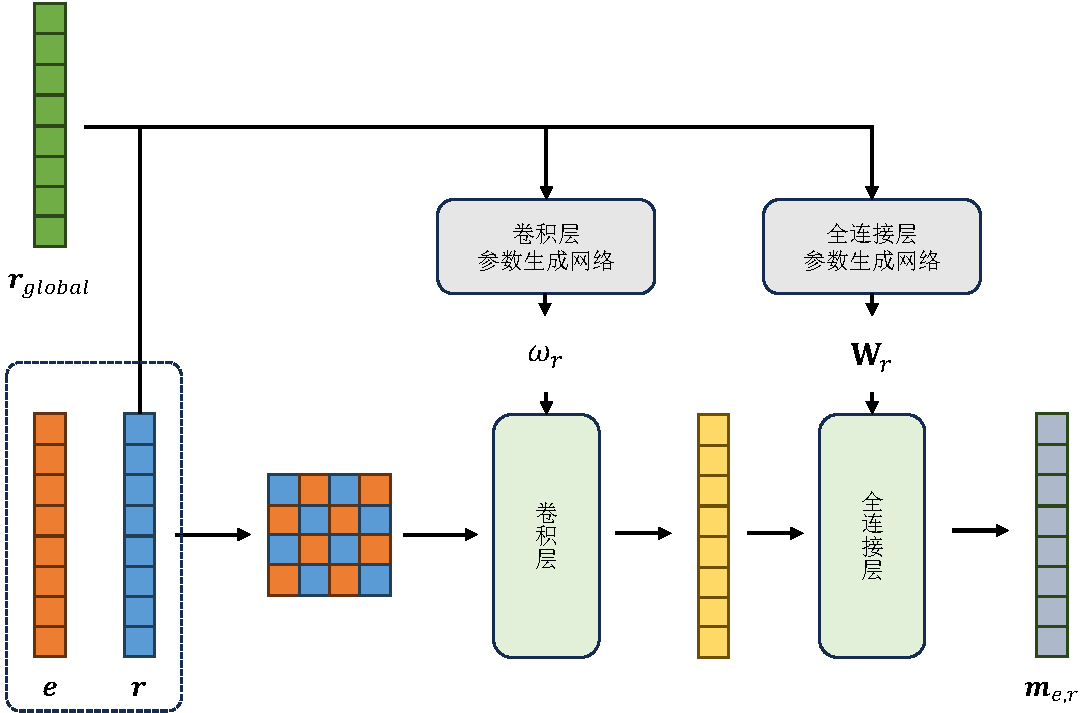
\includegraphics[width=0.75\textwidth]{pic/build_information.pdf}}
  \caption{关系特定的邻居实体信息构造}
  \label{build_information}
\end{figure}

首先,相比于大多数方法采用的实体和关系嵌入拼接之后再线性转换的构造方式,NATLP模型选择将实体和嵌入重塑为二维张量之后再对其进行卷积操作。相比于线性转换,卷积神经网络更擅长捕捉局部模式,通过卷积操作,模型可以有效地提取实体和关系之间的局部交互特征;此外,由于权重共享的特性,卷积神经网络在模型参数上更加高效,使得模型能够用更少的参数完成信息的构建,减少模型过拟合的风险,加快模型训练的过程。而相比于一维卷积,二维卷积能够提升实体和关系嵌入之间的特征交互,从而获得更丰富的特征。为了进一步的提升实体和关系之间的交互,NATLP采用了棋盘式的特征重组方式来进行二维张量的重塑,实体中的每一个特征分量能够和四个关系的特征分量进行交互,如图\ref{cross_conv}所示:

\begin{figure}[htb]
  \centerline{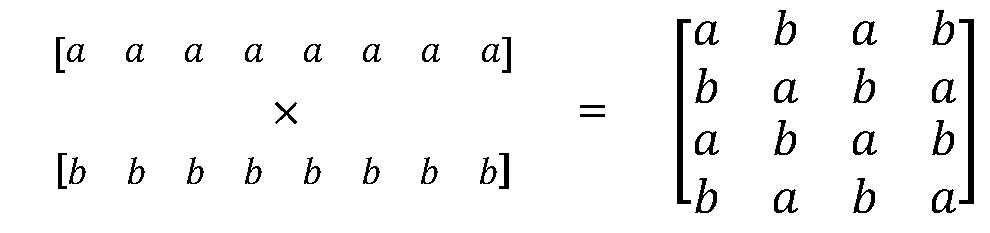
\includegraphics[width=0.8\textwidth]{pic/cross_conv.pdf}}
  \caption{棋盘式特征重组}
  \label{cross_conv}
\end{figure}
% NATLP采用卷积神经网络来完成邻居信息的构造,利用特定关系参数生成网络来为不同关系生成对应的卷积神经网络参数。为了显示的捕捉不同关系之间的共性,NATLP引入了一个全局关系嵌入参与网络参数的生成。

具体的,给定一个邻居实体$e$和相连的关系$r$,模型先采用棋盘式特征重组的方式将实体嵌入和关系嵌入重塑为二维张量:
\begin{equation}
  \phi_{chk}\left(\boldsymbol{e},\boldsymbol{r}\right) 
\end{equation}
其中$\phi_{chk}$代表棋盘式特征重组,$\boldsymbol{e} \in \mathbb{R} ^d$为实体$e$的嵌入表示,$\boldsymbol{r} \in \mathbb{R}^d$为关系$r$的嵌入表示,$d$为嵌入的维度。

将实体和关系嵌入表示重塑为二维张量之后,NATLP会对其进行循环卷积操作:
\begin{equation}
  \phi_{chk}\left(\boldsymbol{e},\boldsymbol{r}\right) \circledast \omega_r
\end{equation}

其中$\circledast$代表循环卷积。相比于普通的卷积操作,循环卷积能够捕捉更多的特征交互。卷积完成后,NATLP将卷积的输出重组为一维向量,再经过线性变化之后就可以得到邻居实体向中心实体传递的信息$\boldsymbol{m}_{e,r} \in \mathbb{R} ^d$:
\begin{equation}
  \boldsymbol{m}_{e,r}=f\left(vec\left(f\left(\phi_{chk}\left(\boldsymbol{e},\boldsymbol{r}\right) \circledast \omega_r \right)\right)\mathbf{W}_r\right)
\end{equation}
其中$f(\cdot )$代表ReLU激活函数,$vec(\cdot)$代表将卷积的输出重整为一维向量的操作。

为了让模型能够充分捕获关系对于实体消息传递的影响,NATLP采用参数生成网络来为卷积层和全连接层生成关系对应的特定参数$\omega_r$和$\mathbf{W}_r$。同时,为了显示地捕捉不同关系之间的共性,NATLP引入了一个全局关系嵌入$\boldsymbol{r}_{global}$参与网络参数的生成:
\begin{gather}
  \omega_r = \mbox{Re3D}\left(\mathbf{W}_{conv}\left[\boldsymbol{r};\boldsymbol{r}_{global}\right]\right) \\
  \mathbf{W}_r = \mbox{Re2D}\left(\mathbf{W}_{fc}\left[\boldsymbol{r};\boldsymbol{r}_{global}\right]\right)
\end{gather}

其中$\mathbf{W}_{conv} \in \mathcal{R}^{n_{conv}\times k_{size} \times k_{size} \times d}$为卷积层参数生成网络,$n_{conv}$为卷积核的数量,$k_{size}$为卷积核的边长,$\mathbf{W}_{fc}$为全连接层参数生成网络,$\mbox{Re3D}(\cdot)$和$\mbox{Re2D}(\cdot)$代表将参数生成网络的输出重整为卷积层和全连接层参数需要的三维张量和二维张量的形式。$\boldsymbol{r}_{global}$为全局关系嵌入。通过全局关系嵌入$\boldsymbol{r}_{global}$,模型能够捕捉到不同关系之间的共同特征,当部分关系种类训练数据较少时,模型通过全局关系嵌入也能获得不错的泛化能力。

\subsection{邻域感知Transformer模块}

完成关系特定的邻居实体信息构造之后,NATLP下一步的任务是利用Transformer模型来挖掘局部邻域蕴含的语义和结构信息,并编码成向量形式,提供给解码器进行解码。

给定一个待遇测的事实三元组$(s,r,?)$,其中头实体即中心实体$s$有$n$个邻居实体,$e_i$、$r_i$为中心实体的邻居实体和对应的相连的关系,有$\forall  i\in\left[1,n\right] $,$(s,r_i,e_i) \in \mathcal{T}^\prime $,则在完成关系特定的邻居实体信息构造之后,邻域感知Transformer模块的输入可以表示为以下形式:
\begin{equation}
      \mathbf{M}_{input}=\left[\boldsymbol{s},\boldsymbol{m}_{e_1,r_1},\boldsymbol{m}_{e_2,r_2},...,\boldsymbol{m}_{e_n,r_n}\right]
\end{equation}
\begin{equation}
  \varPhi \left(e,r\right) = f\left(vec\left(f\left(\phi_{chk}\left(\boldsymbol{e},\boldsymbol{r}\right) \circledast \omega_{r} \right)\right)\mathbf{W}_{r}\right)
\end{equation}
\begin{equation}
    \boldsymbol{m}_{e_i,r_i}=\varPhi \left(e_i,r_i\right)
\end{equation}
% \begin{gather}
%   \mathbf{M}_{input}=\left[\boldsymbol{s},\boldsymbol{m}_{e_1,r_1},\boldsymbol{m}_{e_2,r_2},...,\boldsymbol{m}_{e_n,r_n}\right] \\
%   \varPhi \left(e,r\right) = f\left(vec\left(f\left(\phi_{chk}\left(\boldsymbol{e},\boldsymbol{r}\right) \circledast \omega_{r} \right)\right)\mathbf{W}_{r}\right)\\
%   \boldsymbol{m}_{e_i,r_i}=\varPhi \left(e_i,r_i\right)
% \end{gather}
其中$s$为中心实体的嵌入表示,$\boldsymbol{m}_{e_i,r_i}$为实体$e_i$通过关系$r_i$传递的信息。

此外,为了防止在解码的时候模型对某个特定的输入具有偏向性,模型在输入序列的头部添加了一个特殊的嵌入Class Token,表示为$\boldsymbol{e}_{cls}$。Class Token不基于任意的输入内容,在训练之前进行随机的初始化,并且随着网络的训练不断更新,能够在一定程度上编码整个知识图谱的统计特性。最终,在Transformer的输出中,Class Token对应的输出向量被用作代表整个输入序列的特征表示,传递给解码器。为了帮助模型在Class Token、中心实体嵌入表示和邻居实体传递的消息之间进行区分,受到BERT\upcite{BERT}模型的启发,NATLP为以上三类输入分配了可学习的类型嵌入,则邻域感知Transformer模块的最终输入可以表示为:
\begin{equation}
  \mathbf{M}_{input}^\prime = \left[\boldsymbol{e}_{cls},\boldsymbol{s},\boldsymbol{m}_{e_1,r_1},\boldsymbol{m}_{e_2,r_2},...,\boldsymbol{m}_{e_n,r_n}\right]
\end{equation}
\begin{equation}
  \mathbf{M}_{input} = \mathbf{M}_{input}^\prime + \mathbf{TE}
\end{equation}
% \begin{gather}
%   \mathbf{M}_{input}^\prime = \left[\boldsymbol{e}_{cls},\boldsymbol{s},\boldsymbol{m}_{e_1,r_1},\boldsymbol{m}_{e_2,r_2},...,\boldsymbol{m}_{e_n,r_n}\right]\\
%   \mathbf{M}_{input} = \mathbf{M}_{input}^\prime + \mathbf{TE}
% \end{gather}
其中$\mathbf{TE}$代表可学习的类型嵌入。

在完成输入的构造之后,NATLP将利用Transformer的自注意力机制来学习输入中的信息。原始版本的Transformer的第$i$个输入和第$j$个输入之间的注意力分数$a_{ij}$计算公式为:
\begin{equation}
  \label{attention_score}
  a_{ij}=\frac{(\boldsymbol{m}_iW_Q)(\boldsymbol{m}_jW_K)^T}{\sqrt{d}}
\end{equation}
这样的计算方式给Transformer带来的最大优势是让其具备了捕捉输入中全局信息的能力。在Transformer的每一层中,所有的输入都能够接收并处理来自输入序列中任何位置的信息。然而,这样的方式也带来了副作用:输入序列中的结构信息丢失了,在处理邻居实体传递的信息时,模型无法捕捉到邻居实体之间的直接联系,因此模型需要想办法明确区分不同的位置信息或者分辨不同输入之间的位置相关性。在处理序列数据时,可以采用为不同位置的输入分配不同的位置向量的方法解决这个问题,但这种方法并不适合知识图谱这种非欧结构的数据。

为了让Transformer能够捕获中心实体局部邻域中的图结构数据,本文提出了一种节点距离编码,模型根据节点之间在图谱中的最短距离来辅助计算输入之间的注意力分数。一般来说,实体应该更关注距离较近的其他实体。具体来说,当计算注意力时,模型额外添加一个基于实体节点间最短距离的偏置项:
\begin{equation}
  a_{ij}=\frac{(\boldsymbol{m}_iW_Q)(\boldsymbol{m}_jW_K)^T}{\sqrt{d}}+\frac{1}{dis(e_i,e_j)}
\end{equation}
其中$dis(e_i,e_j)$为知识图谱中实体$e_i$和$e_j$之间的最短路径的距离。通过添加额外的辅助项,距离越近的实体之间计算得到的注意力得分越高。

此外,在公式\ref{attention_score}中注意力分数是基于输入信息之间的语义相关性计算的,但是知识图谱中实体的节点度数也是重要的结构信息,它衡量了实体在知识图谱中的重要性。例如,在社交网络知识图谱中,拥有大量关注者的明星的权重应该更高。因此在注意力计算中,节点度数也应该被纳入考虑。具体来说,NATLP在注意力计算中额外添加一个节点度数的辅助项:
\begin{equation}
  a_{ij}=\frac{(\boldsymbol{m}_iW_Q)(\boldsymbol{m}_jW_K)^T}{\sqrt{d}}+1-\frac{1}{\lg (deg_{e_i})\cdot \lg (deg_{e_j})}
\end{equation}
其中$deg_{e_i}$为实体$e_i$的节点度数。两个实体的节点度数越高,注意力得分越高。通过这样的方式,模型能够在注意力机制中同时捕获语义相关性和节点的重要性。

最终,邻域域感知Transformer模块的自注意力计算方式为:
\begin{equation}
  a_{ij}=\frac{(\boldsymbol{m}_iW_Q)(\boldsymbol{m}_jW_K)^T}{\sqrt{d}}+\frac{1}{dis(e_i,e_j)}+1-\frac{1}{\lg (deg_{e_i})\cdot \lg (deg_{e_j})}
\end{equation}
模型取Transformer最后一层的输出中Class Token对应位置的输出向量$\boldsymbol{T}_{cls}$作为整个编码器的最终输出。


\subsection{基于卷积神经网络的解码器}

解码器的主要任务是根据邻域感知Transformer模块的输出来计算待预测三元组正确的概率,对链路预测任务的效果进行评估。在知识图谱补全任务中,一般采用传统的知识图谱嵌入方法作为解码器,它们结构简单,计算效率高,可解释性强。常见的解码器有基于翻译的方法如TransE\upcite{TransE}、基于张量分解的方法DistMult\upcite{DistMult}以及基于卷积神经网络的方法ConvE\upcite{ConvE}。在这之中性能最好,最常被使用的解码器是ConvE,因此NATLP也采用ConvE作为解码器。

给定待遇测的事实三元组$(s,r,?)$和编码器的输出$\boldsymbol{T}_{cls}$,ConvE解码器先计算得到模型预测的候选实体的嵌入$\boldsymbol{o}_{t}$:
\begin{equation}
  \boldsymbol{o}_{t}=f\left(vec\left(f\left(\left[\boldsymbol{T}_{cls};\boldsymbol{r}\right]\ast \omega\right)\right)\mathbf{W}\right)
\end{equation}
其中$\ast$代表卷积操作。随后对于任意一个候选实体$e_t$,模型将$\boldsymbol{o}_{t}$与$e_t$的嵌入$\boldsymbol{e}_{t}$进行点积后并经过sigmoid激活函数后得到$e_t$正确的概率:
\begin{equation}
  p_{e_t} = \sigma(\boldsymbol{o}_{t}\cdot \boldsymbol{e}_{t}^T)
\end{equation}
其中$\sigma(\cdot)$为sigmoid激活函数。

获得所有候选实体的得分后,模型采用交叉熵损失函数计算任务损失:
\begin{equation}
  L = -\frac{1}{N}\sum\limits_{i}t_ilog(p_i)+(1-t_i)log(1-p_i)
\end{equation}
$t_i$为第i个候选实体组成的三元组是否正确的标签,$p_i$是模型预测的第i个候选实体组成的三元组是否正确的概率。

\section{实验方案设计}

\subsection{实验数据集}
为了对NATLP模型进行评估,本文在两个标准基准数据集FB15k-237\upcite{FB15k-237}和WN18RR\upcite{ConvE}上进行了实验。FB15k-237是开源知识图谱Freebase\upcite{freebase}的子集,存储了有关电影、演员、奖项等等现实世界的常识信息的。WN18RR则是开源知识图谱WordNet\upcite{wordnet}的子集,包含了英文单词中的语义信息,例如同义、反义、单词概念的上下层等多种单词语义关系。为了避免测试集出现逆关系泄露的问题,两个数据集中所有的逆关系都已经被去除。两个数据集的统计数据如表\ref{dataset_statistics}所示,其中训练集用于模型参数训练,验证集用于模型超参数调优,测试集用于模型性能评估。值得注意的是,这两个数据集中的关系数量存在差异,FB15k-237包含了237种Freebase中的不同关系,而WN18RR的关系种类数量为11,总的来说,相比于FB15k-237,WN18RR数据集更加的稀疏。

\begin{table}[htbp]
  \renewcommand\arraystretch{1.5}
  \caption{数据集统计信息}
  \centering
  \begin{tabular}{*{3}{c}}
    \toprule
    数据集 & FB15k-237 & WN18RR\\
    \midrule
    \#实体数量  & 10541 & 40943 \\
    \#关系数量 & 237 & 11\\
    \#训练集数量 & 272115 &86835\\
    \#验证集数量 &17535 &3034\\
    \#测试集数量 &20466 &3134\\
    \#实体平均度数 &42.7 &4.5\\
    \bottomrule
  \end{tabular}
  \label{dataset_statistics}
\end{table}

\subsection{实验评估策略}

知识图谱的链路预测任务被定义为实体排序预测任务。测试集中的每个三元组将在两种不同的场景中进行链路预测评估:给定头实体和关系下的尾实体预测$(s,r,?)$,以及给定尾实体和关系下的头实体预测$(?,r,o)$。在实践中,头实体预测以$(o,r^-1,?)$的形式执行。预测时,待预测的头实体或者尾实体将被每个候选实体替换,并计算每个候选三元组的得分,随后所有的候选三元组将按照分数降序进行排序,以获得基本事实三元组的准确排名,并根据排名来对评估指标进行计算。

在知识图谱补全任务中,平均排名(Mean Rank,MR)、倒数平均排名(Mean Reciprocal Rank,MRR)和前N名百分比(Hits@n)三种评估指标将用来评估模型的性能。假设测试集中待预测三元组的数量为$K$,$rank_i$为第$i$个三元组的正确实体在所有候选实体中的排序位置,则平均排序MR的计算方式为:
\begin{equation}
    MR = \frac{\sum_i rank_i}{K}
\end{equation}
MR代表了所有正确实体的平均排序位置,MR越小,说明正确实体的得分越高,排名越靠前,模型的性能更好。但是MR存在的最大问题则是它对于不同排序位置的预测效果投入的关注是一样的,例如,假设有两个三元组,其中一个三元组的正确实体的排名从105上升到了100,另一个三元组的正确实体的排名从5上升到了1,它们对于MR指标的贡献是一致的。但是,在实验中从5到1的提升一般被认为是更有意义的,平均排名指标MR则忽略了这一点。

平均倒数排名MRR对于这个问题进行了改进,MRR计算的时候正确实体排名的倒数的平均值,而不是排名的平均值,具体计算公式为:
\begin{equation}
    MRR = \frac{1}{K} \sum_i \frac{1}{rank_i}
\end{equation}
通过这样的计算方式,排名越靠前的项会获得更大的权重占比,对于整体性能指标的贡献越大。和MR不同,MRR越高,代表模型的性能越好。

前N名百分比Hits@n指的则是所有测试三元组中正确实体的排序处于前n名的比例,计算方式为:
\begin{equation}
    Hits@n = \frac{\sum_i \left[1 \ if \ rank_i \leq n \ or \ 0\right] }{K}
\end{equation}
指标越高,代表模型的性能越好。在知识图谱补全任务中,常用的前N名百分比指标包括Hits@1,Hits@3和Hits@10。

此外,注意到对于一个待预测的三元组$(s,r,?)$,正确实体$o$的选项可能不止一个,例如(姚明,出生于,上海)和(姚明,出生于,中国)都是正确的事实。在计算评价指标时,其余的正确实体可能会导致当前测试三元组中的正确实体排名下降,对模型评估造成影响,因此本文和大多数基线模型类似,计算排序时除了基本事实三元组之外的所有正确三元组都被排除在排名之外。

\subsection{实验环境}

本文采用的实验环境中的服务器硬件和软件配置如表\ref{environment}所示。硬件配置方面,实验所采用的服务器的处理器规格为Intel(R) Core(TM) i9-10920X CPU @ 3.50GHz,内存大小为128G,使用的显卡型号为GeForce RTX 4090,对应的显存大小为24G;软件配置方面,使用的操作系统为Ubuntu 5.4.0-74,采用的编程语言为Python,版本为3.10.9,使用的深度学习框架及其对应的版本为Pytorch 1.13.1。

\subsection{对比算法}
为了验证本文提出的NATLP方法在知识图谱补全任务上的有效性,实验部分本文选取了一些最具代表性的以及最先进的知识图谱补全方法作为基线模型与NATLP模型进行了对比实验,主要包含以下几类方法:

(1)基于翻译的知识图谱嵌入模型,包括TransE\upcite{TransE},RotatE\upcite{RotatE}。TransE将关系视为头实体到尾实体的翻译过程,RotatE则进一步的将关系拓展为头实体到尾实体的旋转

\begin{table}[htbp]
    \renewcommand\arraystretch{1.5}
    \caption{采用的实验环境}
    \centering
    \begin{tabular}{*{2}{c}}
      \toprule
      配置项目 & 版本/内容\\
      \midrule
      处理器  & Intel(R) Core(TM) i9-10920X CPU @ 3.50GHz \\
      内存 & 128G\\
      显卡 & GeForce RTX 4090\\
      显存 & 24G\\
      操作系统 & Ubuntu 5.4.0-74\\
      编程语言 & Python 3.10.9\\
      深度学习框架 & Pytorch 1.13.1\\
      \bottomrule
    \end{tabular}
    \label{environment}
\end{table}

\noindent
过程。这类方法结构简单,计算速度快,可解释性较强。

(2)基于张量分解的知识图谱嵌入模型,包括DistMult\upcite{DistMult},ComplEx\upcite{ComplEx}。这类方法主要是将将整个知识图谱表示为一个高维的稀疏张量,并通过对其进行张量分解来获得实体和关系的嵌入。DisMult将关系矩阵限制为对角矩阵,压缩了模型参数,ComplEx则将模型从实数域扩展到了复数域,强化了表达能力。和基于翻译的方法类似,这类方法模型结构比较简单,可解释性较强。受限于简单的网络结构,以上两类方法的性能都相对较差。
 
(3)基于卷积神经网络的模型,包括ConvE\upcite{ConvE},ConvR\upcite{ConvR}。ConvE是第一个基于卷积神经网络的知识图谱嵌入方法,将关系和实体嵌入重塑为二维张量并进行卷积来增加特征交互。ConvR则直接使用关系嵌入作为卷积神经网络的卷积核来对实体嵌入进行卷积,减少了网络参数。这类方法的特点是利用卷积神经网络来提高模型的表达能力,并通过优化二维张量的塑造方式增加实体和关系之间的特征交互,缺点是可解释性较差,且和基于翻译和基于神经网络的方法一样,都忽略了知识图谱丰富的图结构信息。

(4)基于图神经网络的知识图谱嵌入模型,这类方法的核心思想是利用图神经网络来学习图谱中的结构信息,获得了很大的性能提升。主要包括基于图卷积神经网络的R-GCN\upcite{R-GCN},CompGCN\upcite{CompGCN},以及基于图注意力网络的KBGAT\upcite{KBGAT},HKGN\upcite{HKGN},SE-GNN\upcite{SE-GNN}和MRGAT\upcite{MRGAT}。这类方法的缺点是采用的聚合方法比较简单,模型的表达能力还有进一步提升的空间。

\subsection{超参数设置}

NATLP模型在实验中采用的超参数是通过网格搜索在验证集上进行评估后得出的,主要涉及到的超参数有实体和关系嵌入的维度、关系特定的邻居实体信息构造中使用的卷积核的大小、卷积核的数量、不同神经网络层的Dropout概率、训练批次的大小、训练中的总迭代次数、训练中的最大学习率以及标签的平滑比例等。

实验中采用了Adamax\upcite{Adamax}优化器结合动态学习率调整策略进行模型的训练。在总迭代次数的前10\%内,模型的学习率将从0线性提升到最高,并在剩余迭代次数内线性下降到0。为了防止模型出现过度自信的现象,训练过程中以0.1的比率进行了标签平滑。NATLP模型在两个数据集上的具体的超参数设置见表\ref{NALTP_hyperparameter}所示。

\begin{table}[htbp]
  \renewcommand\arraystretch{1.5}
  \caption{NATLP模型超参数设置}
  \centering
  \begin{tabular}{*{3}{c}}
    \toprule
    超参数 & FB15k-237 & WN18RR\\
    \midrule
    实体和关系嵌入大小  & 320 & 320 \\
    卷积核大小 & 3$\times$3 & 3$\times$3\\
    卷积核数量 & 32 & 32\\
    Transformer网络层数& 4 & 4\\
    嵌入层Dropout概率 & 0.2 & 0.2\\
    Transformer中的Dropout概率 & 0.6 & 0.6\\
    训练批次大小 & 512 & 512\\
    总迭代次数& 300 & 500 \\
    最大学习率 & 0.001 & 0.02\\
    标签平滑比例 & 0.1 & 0.1\\
    \bottomrule
  \end{tabular}
  \label{NALTP_hyperparameter}
\end{table}

\section{实验结果与分析}

\subsection{整体实验结果分析}

不同模型在WN18RR数据集和FB15k-237数据集上的链路预测实验结果如表\ref{NATLP_result_tab}所示。文献\cite{49}在充分大的超参数搜索空间下采用统一的训练框架进行了大量的实验,探究了不同训练策略、模型架构和超参数搜索方法对于知识图谱嵌入模型性能的影响,发现如果选择合适的训练方法,许多浅层的知识图谱嵌入模型能够获得比原始文献中优秀得多的性能。因此TransE,RotatE,DistMult,ComplEx和ConvE模型在两个数据集上的实验结果直接选取文献\cite{49}中经过大量调参后的最优结果。另外,由于文献\cite{50}指出KBGAT模型中存在评估策略不当以及测试集数据泄露的问题,因此KBGAT的实验结果选取自文献\cite{50}中经过修正后的结果。

\begin{table}[htbp]
  \begin{center}
      \caption{NATLP实验结果}
      \renewcommand\arraystretch{1.5}
      \setlength{\tabcolsep}{5pt}
      \begin{tabular}{*{11}{c}}
          \toprule
          \multirow[vpos]{2}{*}[-0.8ex]{模型} & \multicolumn{5}{c}{WN18RR} & \multicolumn{5}{c}{FB15k-237}\\
          \cmidrule(lr){2-6}\cmidrule(lr){7-11}
          &MRR & MR & Hits@1 &Hits@3 & Hits@10&MRR & MR & Hits@1 &Hits@3 & Hits@10\\
          \midrule
          TransE&0.228&-&0.053&0.368&0.520&0.313&-&0.221&0.347&0.497\\
          RotatE&0.478&-&0.439&0.494&0.553&0.333&	-&0.240&0.368&0.522\\
          \cmidrule{1-11}
          DistMult&0.452&-&0.413&0.466	&0.530	&0.343	&-	&0.250	&0.378	&0.531\\
          ComplEx&0.475&-&0.438	&0.490	&0.547	&0.348	&-	&0.253	&0.384	&0.536\\
          \cmidrule{1-11}
          ConvE&0.442&-&0.411&0.451	&0.504&	0.339	&-&	0.248&	0.369	&0.521\\
          ConvR&0.475&-&0.443&	0.489&	0.537&	0.350&	-&	0.261&	0.385&	0.528\\
          \cmidrule{1-11}
          R-GCN & -&-&-&-&-&0.248&-&0.153&0.258&0.414\\
          CompGCN&0.479&3533&0.443	&0.494	&   0.546&	0.355	&197	&0.264	&0.390&	0.535\\
          KBGAT&0.412&\textbf{1921}&-&	-&	0.554	&0.157	&270	&-&	-&	0.331\\
          SE-GNN&0.484&3211&0.446&	\underline{0.509}&	\underline{0.572}	&\underline{0.365}& \textbf{157}	&\underline{0.271}	&\underline{0.399}	&\underline{0.549}\\
          MRGAT&0.481&-&0.443&0.501&0.568&0.358	&-&0.266&0.386&0.542\\
          HKGN&\underline{0.487}&\underline{2468}&\underline{0.448}&0.505&0.561&\underline{0.365}&194&\underline{0.271}&0.397&0.544\\
          \cmidrule{1-11}
          \textbf{NATLP}&\textbf{0.505}&2687&\textbf{0.465}&\textbf{0.519}&\textbf{0.576}&\textbf{0.374}&\underline{181}&\textbf{0.281}&\textbf{0.411}&\textbf{0.560}\\
          % TKGE-PN&\textbf{0.510}&2540&\textbf{0.467}	&\textbf{0.522}	&\underline{0.590}	&\textbf{0.379}	&160	&\underline{0.288}	&\textbf{0.414}	&\textbf{0.562}\\
          \bottomrule
      \end{tabular}
      \label{NATLP_result_tab}
  \end{center}
\end{table}

表中加粗项为每项指标的最高值,下划线项为每项指标的次高值。从表\ref{NATLP_result_tab}中可以观察到,在两个基准数据集的绝大多数指标上,NATLP都取得了最优的效果,相对于次优结果,在FB15k-237数据集上,NATLP在MRR、Hits@1、Hits@3和Hits@10四个指标上分别取得了3.6\%,3.7\%, 1.9\%, 0.6\%的性能提升;在WN18RR数据集上,NATLP在MRR、Hits@1、Hits@3和Hits@10四个指标上分别取得了2.4\%,3.6\%, 3.0\%和2.0\%的性能提升,这表明相比于基线模型,本文提出的NALTP方法在链路预测任务上有着更好的表现,证明了NATLP模型的有效性。同样使用了注意力机制,相比于HKGN以及MRGAT等基于图神经网络的方法,NATLP有着可观的性能提升,证明了Transformer网络强大的表达能力能够增强模型从知识图谱中挖掘语义信息的能力,说明了Transformer网络结构在在知识图谱嵌入领域的应用潜力。

\subsection{模型关键设计分析}

为了验证NATLP模型中关键设计:关系特定的邻居实体信息构造以及邻域感知Transformer模块的有效性,本文进行了多方面的对比实验来验证关键设计的效果。

首先,为了验证关系特定的邻居实体信息构造中参数生成网络以及全局关系嵌入对于链路预测任务的作用,本文在两个数据集上分别以三种设置进行了消融实验,分别是(1)原始NATLP模型,未对模型进行任何改动;(2)消融了参数生成网络的NATLP模型,同一实体在不同关系下进行信息构造中共享完全相同的网络参数;(3)消融了全局关系嵌入的NATLP模型,参数生成网络仅依赖于关系嵌入进行参数生成。实验结果如表\ref{NATLP_ablation1}所示。

\begin{table}[htbp]
  \begin{center}
      \caption{关系特定的邻居实体信息构造消融实验}
      \setlength{\tabcolsep}{8pt}
      \renewcommand\arraystretch{1.5}
      % \renewcommand{\arraystretch}{1}
      \begin{tabular}{*{7}{c}}
          \toprule
          数据集 & 模型设置 & MRR&MR&Hits@1&Hits@3&	Hits@10\\
          \midrule
          \multirow{3}{*}{WN18RR}&NATLP&0.505&2504&0.466&0.519&0.578\\
          &消融参数生成网络&0.496&2399&0.456&0.512&0.575\\
          &消融全局关系嵌入&0.503&2519&0.461&0.518&0.578\\
          \cmidrule{1-7}
          \multirow{3}{*}{FB15k-237}&NATLP&0.376&161&0.284&0.411&0.561\\
          &消融参数生成网络&0.367&145&0.274&0.404&0.555\\
          &消融全局关系嵌入&0.373&175&0.279&0.411&0.558\\
          \bottomrule
      \end{tabular}
      \label{NATLP_ablation1}
  \end{center}
\end{table}

从表\ref{NATLP_ablation1}中实验结果可以观察到,在对参数生成网络进行消融后,模型的在两个数据集上的链路预测性能都有了明显的下降,这证明了相比于采用统一的网络参数进行消息构造,关系特定的网络参数能够更好地捕捉实体中关系相关的特定特征,挖掘与特定关系相关的语义信息,提高任务性能;另外,注意到消融了参数生成网络之后,相比于WN18RR数据集上的表现,NATLP模型在FB15k-237数据集上的性能下降更为严重,本文认为这样的差异主要是由于两个数据集上的关系种类差异所导致的,FB15k-237数据集中的关系种类为237种,远远超过WN18RR数据集上的11种,各个种类的关系之间差异性较大,因此相对的,不同关系采用相同的网络参数进行编码后,NATLP模型在FB15k-237数据集上损失的信息更多,导致模型性能下降更为严重。此外,可以发现,去除全局关系嵌入后模型在两个数据集上的性能也出现了一定的下滑,证明了通过全局关系嵌入显式地捕捉不同关系之间的共同特征同样有助于提高模型的性能。

此外,为了验证邻域感知Transformer模块中基于实体节点间最短距离的偏置项以及基于节点度数的偏置项的有效性,本文在两个数据集上以四种设置进行了NATLP模型的消融实验,分别是(1)原始NATLP模型,未对模型进行任何改动;(2)消融了基于实体节点间最短距离的偏置项的NATLP模型;(3)消融了基于节点度数的偏置项的NATLP模型;(4)同时对两个偏置项进行了消融的NATLP模型。具体实验结果如表\ref{NATLP_ablation2}所示。

\begin{table}[htbp]
  \begin{center}
      \caption{邻域感知Transformer模块消融实验}
      \setlength{\tabcolsep}{8pt}
      \renewcommand\arraystretch{1.5}
      % \renewcommand{\arraystretch}{1}
      \begin{tabular}{*{7}{c}}
          \toprule
          数据集 & 模型设置 & MRR&MR&Hits@1&Hits@3&	Hits@10\\
          \midrule
          \multirow{4}{*}{WN18RR}&NATLP&0.505&2504&0.466&0.519&0.578\\
          &消融节点最短距离的偏置项&0.500&2603&0.457&0.515&0.573\\
          &消融节点度数偏置项&0.501&2570&0.459&0.517&0.578\\
          &消融两个偏置项&0.497&2856&0.454&0.515&0.570\\
          \cmidrule{1-7}
          \multirow{4}{*}{FB15k-237}&NATLP&0.376&161&0.284&0.411&0.561\\
          &消融节点最短距离的偏置项&0.373&180&0.280&0.409&0.557\\
          &消融节点度数偏置项&0.372&184&0.281&0.409&0.554\\
          &消融两个偏置项&0.369&179&0.277&0.409&0.550\\
          \bottomrule
      \end{tabular}
      \label{NATLP_ablation2}
  \end{center}
\end{table}

通过表中结果可以发现,无论是消融了节点间最短距离的偏置项还是节点度数的偏置项,模型在两个数据集上的性能均出现了一定的下滑,证明了通过自注意力计算过程中两个基于知识图谱结构信息的偏置项,邻域感知Transformer模块能够实现对知识图谱图结构的有效感知,提高模型的知识图谱补全性能。


\section{本章小结}

本章对NATLP模型的整体架构、实现细节以及相关的实验与验证部分进行了详细的介绍。本章首先介绍了当前基于图神经网络的方法存在的部分问题以及Transformer在知识图谱嵌入领域中应用的限制;随后给出了模型中涉及到的数学符号的详细定义;之后介绍了模型的整体架构组成;最后,对NATLP中的关键设计细节进行了具体的说明,包括(1)关系特定的邻居实体信息构造,利用参数生成网络生成关系特定的网络参数,学习关系对于实体信息传递的作用,并利用全局关系嵌入捕捉不同关系之间的共性。(2)邻域感知Transformer模块,通过最短距离编码和度数编码在自注意力机制计算时融合图结构信息,捕捉邻居消息之间的互相依赖,更好地适应知识图谱的图结构形式。(3)基于卷积神经网络的解码器,利用基于卷积神经网络的方法ConvE进行解码,并计算任务的交叉熵损失。
而在实验部分,本文首先对实验的基本方案设计进行了说明,包括实验采用的数据集,模型的评估策略以及实验的硬件和软件环境,并介绍了用来对比NATLP的基线模型。随后论文对NALTP模型的整体实验结果进行了介绍,相对于次优结果,在FB15k-237数据集上,NATLP在MRR、Hits@1、Hits@3和Hits@10四个指标上分别取得了3.6\%,3.7\%, 1.9\%, 0.6\%的性能提升;在WN18RR数据集上,NATLP在MRR、Hits@1、Hits@3和Hits@10四个指标上分别取得了2.4\%,3.6\%, 3.0\%和2.0\%的性能提升,证明了NATLP模型的性能表现优于绝大部分现有的模型;最后通过消融实验对NATLP模型中的关键设计:关系特定的邻居实体信息构造以及邻域感知Transformer模块进行了深入的探究和分析,证明了通过显式捕捉关系对于实体消息传递的影响,以及在自注意力机制中编码知识图谱图结构能够有效地提高模型的链路预测任务性能。